\chapter{Systémy rozpoznávania reči} \label{cha:asr-systems}

Nakoľko hodnotenie výslovnosti je vo väčšine prípadov založené na automatickom rozpoznávaní reči (ASR, z~angl. \textit{Automatic Speech Recognition}), v~tejto kapitole si bližšie priblížime fungovanie systémov rozpoznávania reči a ich základné časti. Text tejto kapitoly vychádza z~nasledovných publikácii \cite{Psutka2006, Gales2007, Young2015, Dong2015}.

Pod problémom rozpoznávania reči rozumieme hľadanie najpravdepodobnejšej postupnosti slov, ktorá zodpovedá danému rečovému signálu. Naším cieľom je teda nájsť takú postupnosť slov $\hat{W} = (w_1, w_2, \dots, w_K)$, pre ktorú je aposteriórna pravdepodobnosť $P(W | \bm{O})$ maximálna a kde $\textbf{O} = (\bm{o}_1, \bm{o}_2, \dots, \bm{o}_T)$ je rečový signál vo forme vektoru príznakov, viď sekciu \ref{sec:feature-extraction}. Túto úlohu je však obtiažne riešiť priamo a preto s~využitím Bayesovho teorému definujme ekvivalentný problém

\begin{equation}
    \hat{W} = \argmax_W p(\bm{O} | W) P(W), \label{eq:asr-max-word-sequence}
\end{equation}

\noindent kde $\hat{W}$ je najpravdepodobnejšia postupnosť slov. K~určeniu vierohodnosti $p(\bm{O} | W)$ sa používa tzv. akustický model, ktorý nesie informáciu o~tom, ako znejú jednotlivé fonémy. Pravdepodobnosť $P(W)$ sa stanovuje pomocou jazykového modelu, ktorý nám poskytuje informáciu o~tom, ktoré postupnosti slov sú v~danom jazyku pravdepodobné.
Výsledný systém rozpoznávania reči je potom možné rozdeliť do niekoľkých častí ako je to znázornené na obr.\,\ref{fig:asr-diagram}. V~nasledujúcich sekciách si fungovanie jednotlivých častí bližšie popíšeme.

\begin{figure}
    \centering
    % \includegraphics[width=0.9\textwidth]{figures/asr-diagram.png}
    \newif\ifstandalone
\standalonetrue % comment out for compilation with ktikz	

\ifstandalone
\documentclass{standalone}
\fi

\usetikzlibrary{shapes.geometric, arrows, positioning, arrows.meta, calc}

\ifstandalone
\begin{document}
\fi

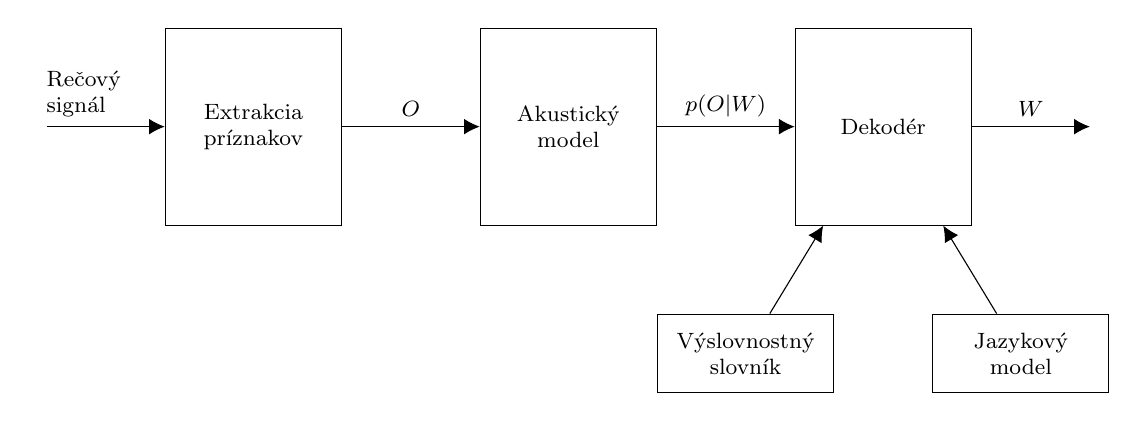
\begin{tikzpicture}[every node/.style = {font=\footnotesize}, node distance=4cm, >={Latex[width=2mm,length=2mm]}]
		\tikzstyle{block} = [rectangle, minimum width=2cm, minimum height=2.5cm, text centered, text width=2cm, draw=black]
		\tikzstyle{small block} = [block, minimum height=1cm]
		%\tikzstyle{arrow} = [thick,->,>=stealth]
		\tikzstyle{arrow} = [->]

		%\node[io](speech){Rečový signál};
		\node[block](fe){Extrakcia príznakov};
		\node[left=1.5cm of fe] (input) {};
		\node[block, right of=fe](am){Akustický model};
		\node[block, right of=am](decoder){Dekodér};
		\node[right=1.5cm of decoder](output) {};
		\node[below=1.5cm of decoder](dummy){};
	    \node[small block, left=0.5cm of dummy] (lexicon) {Výslovnostný slovník};
		\node[small block, right=0.5cm of dummy](lm){Jazykový model};

		\draw[arrow] (input) -- (fe) node[midway, above, text width=1.5cm, align=flush left] {Rečový signál};
		\draw[arrow] (fe) -- (am) node[midway, above] {$\bm{O}$};
		\draw[arrow] (am) -- (decoder) node[midway, above] {$p(\bm{O}|W)$};
		\draw[arrow] (lexicon) -- (decoder);
		\draw[arrow] (lm) -- (decoder);
		\draw[arrow] (decoder) -- (output) node[midway, above] {$W$};
        %\node[io, text centered, above=0.5cm of am] (am-input) {KANONICKÝ PREPIS};
        %\node[io, right=0.5cm of am] (am-output) {FONÉMOVÉ ZAROVNANIA};
        %\node[below=0.5cm of am] (dummy) {};
       % \node[block, below=0.5cm of dummy] (fe) {EXTRAKCIA PRÍZNAKOV};
        %\node[io, right=0.5cm of fe] (fe-output) {PRÍZNAKY};
        %\node[block, right=7cm of dummy] (md) {DETEKCIA NESPRÁVNEJ VÝSLOVNOSTI};
        %\draw[arrow] (am) -- (am-output);
        %\draw[arrow] (am-input) -- (am);
        %\draw[arrow] (am-output) -| (md);
        %\draw[arrow] (fe) -- (fe-output);
        %\draw[arrow] (fe-output) -| (md);
\end{tikzpicture}

\ifstandalone
\end{document}
\fi
    \caption{Základné časti systému pre rozpoznávanie reči.}
    \label{fig:asr-diagram}

\end{figure}

\section{Extrakcia príznakov} \label{sec:feature-extraction}

Úlohou extrakcie príznakov je previesť rečový signál do podoby, ktorá je vhodná pre následné rozpoznávanie. Primárnou snahou je odstrániť prebytočnú informáciu, ktorú nesie pôvodný signál. Ďalšie požiadavky na vlastnosti príznakov vyplývajú z~použitého akustického modelu. 
Samotný výpočet príznakov potom prebieha nad krátkymi, čiastočne sa prekrývajúcimi úsekmi reči. 

Medzi najpoužívanejší typ príznakov patria melovské kepstrálne koeficienty (MFCC) \cite{Davis1980}. Tieto
príznaky sa snažia zohľadňovať nelineárne vnímanie frekvencií ľudským uchom 
s~využitím tzv. melovej frekvenčnej škály. Algoritmus výpočtu pozostáva z~určenia spektrálnych energií pomocou diskrétnej Fourierovej transformácie, váhovania pomocou banky filtrov rozmiestnených v~melovej frekvenčnej škále, logaritmovania získaných hodnôt a nakoniec aplikovania diskrétnej kosínusovej transformácie (\textit{Discrete Cosine Transform}, DCT).

Na podobnom princípe sú založené aj perceptívne lineárne prediktívne (\textit{Perceptual Linear Predictive}, PLP) koeficienty \cite{Hermansky1990}, ktoré v~porovnaní s~MFCC dosahujú v~niektorých prípadoch nepatrne lepšie výsledky \cite{Woodland1997}.

Pri akustických modeloch založených na neurónových sieťach sa okrem vyššie zmienených príznakov zvyknú používať aj tzv. Fbank príznaky, ktoré sa líšia
od MFCC len vo vynechaní diskrétnej kosínusovej transformácie.
Mohamed a kol. \cite{Mohamed2012} dosiahli pri ich použití značné zlepšenie v~porovnaní s~MFCC.

% TODO delta + delta features

\section{Akustický model}

Základnou jednotkou, ktorú reprezentuje akustický model je fonéma. Preto je pre
určenie vierohodnosti $p(\bm{O}| W)$ postupnosti slov $W = (w_1, w_2, \dots, w_K)$ potrebné každé slovo $w_k$ dekomponovať na postupnosť foném. K~tomuto účelu slúži výslovnostný slovník, ktorý pre každé slovo jazyka obsahuje informáciu o~jeho výslovnosti vo forme fonetického prepisu na fonémy. Jedno slovo však môže mať viacej variant výslovnosti, čo vedie na k~nasledovnému výpočtu vierohodnosti

\begin{equation} \label{eq:word-prob-computation}
    p(\bm{O}| W) = \sum_Q p(\bm{O}|Q) p(Q|W),
\end{equation}

\noindent kde suma je nad všetkými možnými výslovnosťami reťazca $W$, t.j. každé $Q$ je postupnosť výslovností slov $Q = ( Q_1, Q_2, \dots, Q_K )$, pričom každé $Q_k$ je postupnosť foném $Q_k = ( q_1, q_2, \dots, q_m )$. Potom

\begin{equation}
    p(Q|W) = \prod_{k=1}^K p(Q_k|w_k),
\end{equation}

\noindent kde $p(Q_k|w_k)$ je pravdepodobnosť, že slovo $w_k$ je vyslovené ako postupnosť foném $Q_k$. V~praxi sa suma v~rovnici (\ref{eq:word-prob-computation}) často aproximuje pomocou maxima. 

\subsection*{Skryté Markovove modely}

Akustické modelovanie s~využitím skrytých Markovových modelov (\textit{Hidden Markov Model}, HMM) je založené na predpoklade, že postupnosť príznakových vektorov $\bm{O} = ( \bm{o}_1, \bm{o}_2, \dots, \bm{o}_T )$ je generovaná pomocou nejakého skrytého Markovovho modelu. Skrytý Markovov model môžeme chápať ako konečný automat pozostávajúci zo stavov $s_i$ a pravdepodobnostných prechodov $a_{ij}$ medzi jednotlivými stavmi $s_i$ a $s_j$. Pri prechode do stavu $s_j$ v~čase $t$ je zároveň generovaný príznakový vektor $\bm{o}_t$ pomocou rozdelenia pravdepodobnosti $b_j(\bm{o}_t)$, ktorá zodpovedá tomuto stavu. 

Ako sme už spomenuli, základnou jednotku, ktorú modelujeme, je fonéma. Jedna fonéma býva zvyčajne reprezentovaná pomocou topológie znázornenej na obrázku \ref{fig:hmm-phone}. Okrem foném je však zväčša potrebné modelovať aj krátke medzislovné pauzy, obr. \ref{fig:hmm-sp}, a dlhšie trvajúce ticho, obr. \ref{fig:hmm-sil}, ktoré je typické zväčša pre začiatok a koniec viet. Model odpovedajúci nejakej postupnosti slov $W$ je potom možné skonštruovať zreťazením takýchto topológii za seba.

\begin{figure}
    \begin{subfigure}{.5\textwidth}
        \centering
        \includegraphics[width=\linewidth]{figures/hmm-phone.png}   
        \caption{model fonémy}
        \label{fig:hmm-phone}
    \end{subfigure}
    \begin{subfigure}{.5\textwidth}
        \centering
        \includegraphics[width=\linewidth]{figures/hmm-sp.png}   
        \caption{model krátkej pauzy}
        \label{fig:hmm-sp}
    \end{subfigure}
    \begin{subfigure}{.5\textwidth}
        \centering
        \includegraphics[width=\linewidth]{figures/hmm-sil.png}   
        \caption{model ticha}
        \label{fig:hmm-sil}
    \end{subfigure}
    \caption{Topológie rôznych HMM modelov, ktoré pozostávajú z~neemitujúcich počiatočných a koncových stavov, emitujúcich stavov medzi nimi a orientovaných prechodov medzi týmito stavmi.}
    \label{fig:hmm-topology}
\end{figure}

Vierohodnosť sekvencie príznakov $\bm{O}$ pre daný model $M$ a danú postupnosť stavov $S$ zodpovedá vzťahu

\begin{equation}
    p(\bm{O} | M, S) =  a_{s(0)s(1)} \prod_{t=1}^T b_{s(t)}(\bm{o}_t) a_{s(t)s(t+1)},
\end{equation}

\noindent kde stavy $s(0)$, resp. $s(T+1)$, predstavujú počiatočný a koncový stav, ktoré negenerujú žiadny výstupný vektor.
Nakoľko je však postupnosť stavov $S$ skrytá, pre určenie vierohodnosti $p(\bm{O} | M)$ musíme uvažovať všetky možné sekvencie stavov $S$. Dostávame teda

\begin{equation}
    p(\bm{O} | M) = \sum_S p(\bm{O} | M, S).
\end{equation}

\noindent Nakoľko nás pri rozpoznávaní reči zaujíma zväčša len najpravdepodobnejšia postupnosť stavov pre danú sekvencia príznakov, môžeme zaviesť nasledovnú aproximáciu

\begin{equation}
    \hat{p}(\bm{O} | M) = \max_S \left\{ a_{s(0)s(1)} \prod_{t=1}^T b_{s(t)}(\bm{o}_t) a_{s(t)s(t+1)} \right\}.
\end{equation}

\noindent Takýto problém je možné riešiť pomocou Viterbiho algoritmu \cite{Rabiner1989}, ktorý je schopný určiť najpravdepodobnejšiu postupnosť $S$ a teda aj maximálnu hodnotu vierohodnosti. 

Posledným detailom, ktorý sme doposiaľ prehliadali je určenie prechodových pravdepodobností $a_{ij}$ a rozdelenia výstupných pravdepodobností $b_j$. Pre modelovanie $b_j$ sa v~minulosti často používal model zmesí normálnych rozložení (\textit{Gaussian Mixture Model}, GMM). V~súčasnosti však býva nahrádzaný neurónovými sieťami, ktoré sú schopné dosahovať výrazne lepších výsledkov. GMM sa potom využíva len na určenie zarovnaní, na ktorých trénujeme neurónovú sieť, ako tomu bude aj v~tejto práci. Preto nebudeme popisovať samotný algoritmus trénovania $a_{ij}$ a $b_j$, ktorý je pomerne rozsiahly. Dobrý popis je možné nájsť napr. v~\cite{Rabiner1989}.

% \subsection{Neurónové siete} \label{sec:neural-networks}
\section{Jazykový model} \label{sec:language-model}

Ďalšou dôležitou časťou pri rozpoznávaní reči je jazykový model, ktorého úlohou
je pre ľubovoľnú postupnosť slov $W = (w_1, w_2, \dots, w_K)$ určiť aposteriórnu pravdepodobnosť $P(W)$, ktorá je daná vzťahom

\begin{equation} \label{eq:lm-posterior-prob}
    P(W) = \prod_{k=1}^{K} P(w_k | w_{k-1}, \dots, w_1).
\end{equation}

\noindent Jednotlivé podmienené pravdepodobnosti v~rovnici (\ref{eq:lm-posterior-prob}) je potrebné odhadnúť z~trénovacích dát, čo bude s~narastajúcou dĺžkou $K$ postupnosti $W$ čím ďalej tým náročnejšie, až takmer nemožné. Tento problém sa snažia riešiť $N$-gramové jazykové modely, ktoré sú zároveň najpoužívanejšími modelmi používanými k~jazykovému modelovaniu.

$N$-gramové jazykové modely riešia uvedený problém aproximáciou, pri ktorej sú pravdepodobnosti v~(\ref{eq:lm-posterior-prob}) podmienené len $N-1$ poslednými slovami, t.j. dostávame 

\begin{equation} \label{eq:lm-posterior-prob2}
    P(W) = \prod_{k=1}^{K} p(w_k | w_{k-1}, w_{k-2}, \dots, w_{k-N+1}),
\end{equation}

\noindent pričom hodnota $N$ je zvyčajne v~rozmedzí $2$\,--\,$3$. K~odhadu podmienených pravdepodobností potom postačuje nad trénovacími dátami určovať počty výskytov postupností slov, napr. pre $N=3$ je odhad daný vzťahom

\begin{equation}
    p(w_k| w_{k-1}, w_{k-2}) \approx \frac{C(w_{k-2}, w_{k-1}, w_k)}{C(w_{k-2}, w_{k-1})},
\end{equation}

\noindent kde $C(w_{k-2}, w_{k-1}, w_k)$ je počet trigramov $w_{k-2} w_{k-1} w_k$ a $C(w_{k-2}, w_{k-1})$ je počet bigramov $w_{k-2} w_{k-1}$ nachádzajúcich sa v~trénovacích dátach.

Napriek obmedzenej histórii dochádza pri týchto modeloch k~problému s~nedostatkom trénovacích dát, a to napriek tomu, že k~trénovaniu postačujú dáta len v~textovej podobe. K~jeho riešeniu je možné použiť napr. ústupové (\textit{backing-off}) vyhladzovanie. Pre viac informácii viď \cite{Psutka2006}.


\section{Dekódovanie} \label{sec:decoding}

Ako sme si už uviedli v~úvode, cieľom rozpoznávania je nájdenie najpravdepodobnejšej postupnosti slov $\hat{W} = (w_1, w_2, \dots, w_K)$ v~súlade so vzťahom (\ref{eq:asr-max-word-sequence}). Ak by sme však postupovali spôsobom uvedeným vyššie, t.j. určovali by sme hodnoty $p(\bm{O}|W)$ a $P(W)$ pre každú prípustnú postupnosť slov $W$, už pri malom slovníku by bol výpočet nerealizovateľný.
Z~tohto dôvodu bola od počiatku snaha o~hľadanie efektívnejšieho spôsobu dekódovania. 

Rozšíreným spôsobom dekódovania je v~dnešných systémoch rozpoznávania reči používanie ohodnotených konečných transducerov (\textit{Weighted Finite-State Transducer}, WFST), čo je v~podstate konečný automat s~ohodnotenými hranami, ktorý umožňuje nielen čítanie symbolov, ale aj ich generovanie. Veľkou výhodou tohto výpočetného modelu je možnosť reprezentácie všetkých spomenutých častí potrebných pre dekódovanie, t.j. 

\begin{itemize}
    \item skrytý Markovov model transducerom $H$,
    \item výslovnostný slovník transducerom $L$,
    \item jazykový model transducerom $G$.
\end{itemize}

\noindent Potom s~využitím operácií kompozície, determinizácie a minimizácie sme schopný jednotlivé transducery skomponovať do výsledného transduceru $\textit{HLG}$. Takouto kombináciou sme dosiahli výraznej redukcie stavového priestoru, ktorý je potrebné počas dekódovania prehľadávať. Pre samotné dekódovanie je potom možné použiť napr. Viterbiho paprskové (\textit{beam}) dekódovanie. Pre viac informácii o~použití WFST pre rozpoznávanie reči viď \cite{WFST}.
